% !TEX program = xelatex

\documentclass[12pt,a4paper]{article}
\usepackage[UTF8]{ctex}
\usepackage{float}
\usepackage{amsmath}
\usepackage{enumerate}
\usepackage{booktabs}
\usepackage{graphicx}
\usepackage{longtable}
\usepackage{subfigure}

\usepackage{url}
\usepackage{multirow}

% for plotting 
\usepackage{caption}
\usepackage{pgfplots}

% for pseudo code 
\usepackage{algorithm}
\usepackage[noend]{algpseudocode}

% for reference 
\usepackage{hyperref}
\usepackage{cleveref}

% for code 
\usepackage{listings}
\usepackage{xcolor}
\usepackage{fontspec}
\definecolor{darkgreen}{rgb}{0,0.6,0}
\newfontfamily\consolas{Consolas}

\lstset {
    basicstyle=\footnotesize\consolas, % basic font setting
    breaklines=true, 
    frame=single,     % {single, shadowbox, bottomline}
    keywordstyle=\color{blue}, 
    commentstyle=\color{darkgreen},
    stringstyle=\color{red},
    showstringspaces=false,
    % backgroundcolor=\color{black!5}, % set backgroundcolor
    numbers=left, 
    numberstyle=\ttfamily,
}

% Microsoft Word A4 paper default layout 
\usepackage[a4paper, left=3.18cm, right=3.18cm, top=2.54cm, bottom=2.54cm]{geometry}

% \captionsetup[figure]{labelfont={bf}, name={Figure}}
% \captionsetup[table]{labelfont={bf}, name={Table}}

\crefname{equation}{方程}{方程}
\Crefname{equation}{方程}{方程}
\crefname{table}{表}{表}
\Crefname{table}{表}{表}
\crefname{figure}{图}{图}
\Crefname{figure}{图}{图}

\title{数学实验:第二次作业}
\author{计算机系 \quad 计73 \quad 2017011620 \quad 李家昊}
\date{\today}

% 实验报告格式的基本要求

% 系别、班级、学号、姓名

% 1 实验目的
% 2 题目
%   2.1 计算题:题号,算法设计(包括计算公式),程序,计算结果(计算机输出),结果分析,结论。
%   2.2 应用题:题号,问题分析,模型假设,模型建立,算法设计(包括计算公式),程序,计算结果(计算机输出),结果的数学分析,结果的实际意义,结论。
% 3 收获与建议

\begin{document}

\maketitle

\section{实验目的}

\begin{itemize}
    \item 掌握用MATLAB 软件求微分方程初值问题数值解的方法
    \item 通过实例学习用微分方程模型解决简化的实际问题
    \item 了解欧拉方法和龙格-库塔方法的基本思想和计算公式,及稳定性等概念
    \item 练习数值微分的计算
\end{itemize}

\section{问题求解}

\subsection{Chap4-Ex5 放射性废物的处理(应用题)}

\subsubsection{问题分析}

题目给定装有放射性废物圆桶的体积,重量,所受海水浮力,海水阻力,最大撞击速度等参数,求圆桶撞击海底时会不会破裂。

\subsubsection{模型假设}

考虑到实际情况,此模型基于以下假设,
\begin{enumerate}[1.]
    \item 圆桶紧贴水面以零初速度自由下落。
    \item 圆桶下落过程中仅受浮力,重力,以及海水阻力的作用。
    \item 海水的密度不随深度变化,即海水对圆桶的浮力不变。
\end{enumerate}

\subsubsection{模型建立}

设圆桶的质量为$m$,重力加速度为$g$,所受浮力固定为$F$,海水阻力系数为$k$,圆桶在$t$时刻下沉速度为$v(t)$,根据牛顿第二定律得到下列微分方程,
\begin{equation}\label{eq:ex5_model}
    mg - F - kv = m \frac{dv}{dt}
\end{equation}
不妨假设物体在$t=0$时刻自由落体投入水中,即$v(0) = 0$,作为微分方程的初值条件。

\subsubsection{算法设计}

\paragraph{解析解法}

根据\Cref{eq:ex5_model}得出通解为,
\begin{equation}
    v(t) = \frac{1}{k}\left(mg - F - Ae^{-\frac{k}{m}t}\right)
\end{equation}
带入初值条件$v(0)=0$,解得系数$A=mg - F$,得到特解,
\begin{equation}\label{eq:ex5_velocity}
    v(t) = \frac{mg -F}{k}\left(1-e^{-\frac{k}{m}t}\right)
\end{equation}
设圆桶在$t_m$时刻达到最大承受速度$v_m$,根据\Cref{eq:ex5_velocity}解得,
\begin{equation}
    t_m = \frac{m}{k}\ln\left(1 + \frac{kv_m}{mg - F - kv_m}\right)
\end{equation}
设圆桶在$t$时刻下落距离为$s(t)$,则有,
\begin{equation}
    s(t) = \int_{0}^{t} v(\tau) d\tau = \frac{mg - F}{k}\left(t + \frac{m}{k}e^{-\frac{k}{m}t}-\frac{m}{k}\right)
\end{equation}
设海水深度为$s_m$,若$s(t_m) < s_m$,则说明圆桶到达海底之前,速度已经达到$v_m$,因此圆桶撞击海底时将破裂;否则,圆桶将不会破裂。

带入题目提供的数据,$g=9.80665\ \mathrm{m/s^2}=32.17405\ \mathrm{ft/s^2}$,$mg=527.436\ \mathrm{lb}$,$F=470.327\ \mathrm{lb}$,$k=0.08\ \mathrm{lb \cdot s / ft}$,$v_m = 40\ \mathrm{ft/s}$,$s_m=300\ \mathrm{ft}$,解得$t_m = 11.8163\ \mathrm{s}$,$s(t_m) = 238.5968\ \mathrm{ft}$,因此有$s(t_m) < s_m$,圆桶撞击海底时将破裂,工程师赢得了官司。

\paragraph{数值解法}

模型需要求解\Cref{eq:ex5_model},为非刚性方程,可利用Matlab内置的5级4阶 Runge-Kutta 方法\texttt{ode45}求解。

\subsubsection{Matlab程序}

请参见\Cref{sec:ex5_code}。

\subsubsection{计算结果}

圆桶的速度和深度随时间变化的图像如\Cref{fig:ex5_result}所示,截取圆桶临近海底时的数值结果如\Cref{tab:ex5_detail}所示,可以看出,圆桶撞击海底的时刻约为$t=13.3\ \mathrm{s}$,速度约为$v=44.8\ \mathrm{ft/s}$,大于圆桶的最大承受速度$v_m = 40\ \mathrm{ft/s}$。

\begin{table}[t]
    \centering
    \caption{圆桶临近海底时的时刻,速度和深度的数值结果。}
    \label{tab:ex5_detail}
    \begin{tabular}{ccc}
        \toprule
        Time (s) & Velocity (ft/s) & Depth (ft)\tabularnewline
        \midrule
        13.0000 & 43.8814 & 288.2447\tabularnewline
        13.1000 & 44.2083 & 292.6492\tabularnewline
        13.2000 & 44.5350 & 297.0864\tabularnewline
        13.3000 & 44.8616 & 301.5562\tabularnewline
        13.4000 & 45.1880 & 306.0587\tabularnewline
        13.5000 & 45.5142 & 310.5938\tabularnewline
        \bottomrule
    \end{tabular}
\end{table}

\begin{figure}[t]
    \centering
    \subfigure[速度随时间变化图像]{
        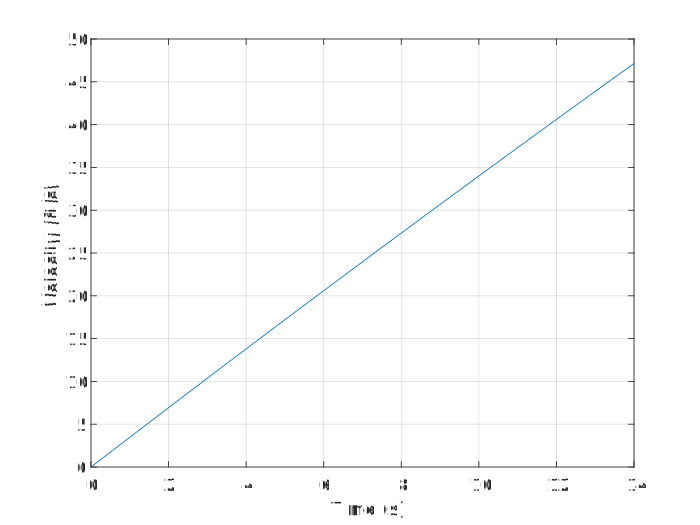
\includegraphics[width=0.47\textwidth]{fig/ex5_velocity.pdf}
    }
    \subfigure[深度随时间变化图像]{
        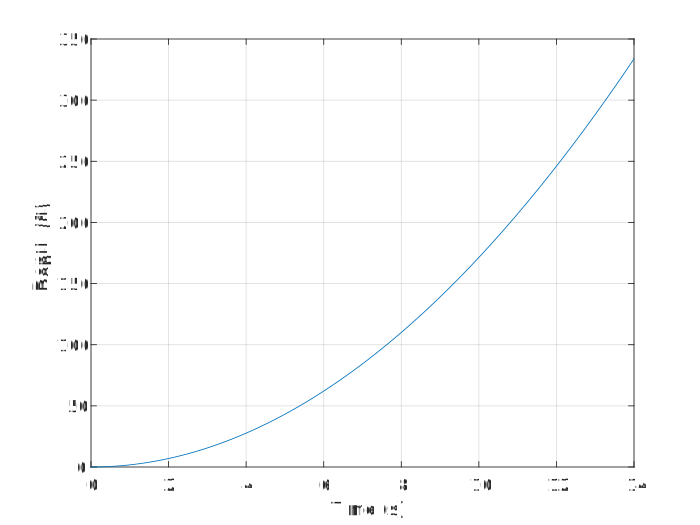
\includegraphics[width=0.47\textwidth]{fig/ex5_depth.pdf}
    }
    \caption{圆桶的速度和深度随时间变化的图像}
    \label{fig:ex5_result}
\end{figure}

\subsubsection{结果的数学分析}

为了分析微分方程数值解法的误差,设圆桶速度的解析解为$v(t)$,数值解为$v^*(t)$,则在数值解法的离散点处作出$v^*(t) - v(t)$的残差图像,如\Cref{fig:ex5_residual}所示。可见,在$t\in[0,14]$范围内,圆桶速度的绝对误差控制在$10^{-11}\ \mathrm{ft/s}$以内;撞击海底时,圆桶速度的相对误差控制在$10^{-12}$以内,数值计算的结果十分精确,可作为最终的计算结果。

\begin{figure}[t]
    \centering
    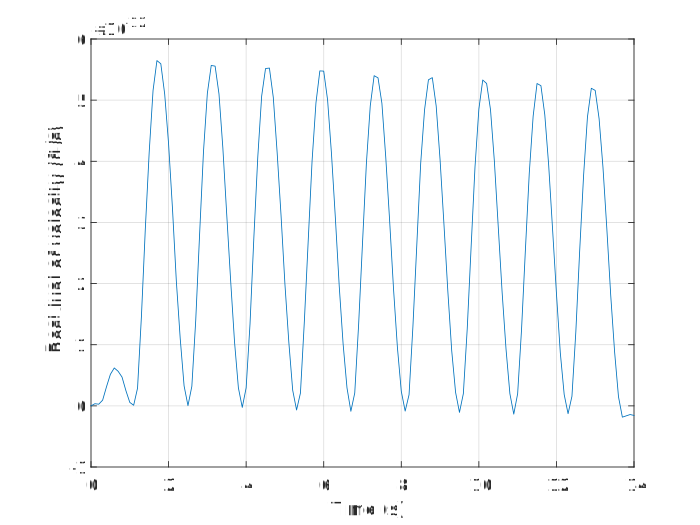
\includegraphics[width=0.8\textwidth]{fig/ex5_residual.pdf}
    \caption{圆桶速度的数值解与解析解之间的残差图像}
    \label{fig:ex5_residual}
\end{figure}

\subsubsection{结果的实际意义}

圆桶大约以$44.8\ \mathrm{ft/s}$的速度撞击海底,并发生破裂,工程师将赢得官司。

\subsubsection{结论}

圆桶撞击海底时会发生破裂,工程师赢得了官司。

\subsection{Chap4-Ex6 小船过河(计算题)}

\subsubsection{算法设计}

\paragraph{数学模型} 以$A$为原点,以$v_1$方向为$x$轴正方向,$\overrightarrow{AB}$方向为$y$轴正方向,建立平面直角坐标系,则有坐标$A(0,0)$,$B(0,d)$,设在$t$时刻,船的坐标为$C(x,y)$,设$\angle ABC = \theta$,则可列出微分方程组,
\begin{equation}\label{eq:ex6_dxy_dt}
    \dfrac{dx}{dt} = v_1 - v_2 \sin \theta, \quad \dfrac{dy}{dt} = v_2 \cos \theta
\end{equation}
消掉$t$,带入题目条件$k=v_1/v_2$,得到,
\begin{equation}\label{eq:ex6_dy_dx}
    \frac{dx}{dy} = \frac{v_1 - v_2 \sin \theta}{v_2 \cos \theta} = \frac{k-\sin \theta}{\cos \theta}
\end{equation}
其中$\theta$满足,
\begin{equation}
    \cos \theta = \frac{d-y}{\sqrt{x^2 + (d-y)^2}}, \quad \sin \theta = \frac{x}{\sqrt{x^2 + (d-y)^2}}
\end{equation}
带入\Cref{eq:ex6_dy_dx}得到,
\begin{equation}\label{eq:ex6_model}
    \frac{dx}{dy} = \frac{k\sqrt{x^2 + (d-y)^2} - x}{d - y}
\end{equation}
即为模型对应的微分方程,对于初值,由于小船从$A(0,0)$出发,因此有$x(0) = 0$。

\paragraph{解析解法} 设$p = x/(d-y)$,则有,
\begin{equation}
    \frac{dp}{dy} = \frac{1}{(d-y)^2}\left(\frac{dx}{dy}(d-y)+x\right) = \frac{1}{d-y}\left(\frac{dx}{dy} + p\right)
\end{equation}
带入\Cref{eq:ex6_model}得到,
\begin{equation}
    (d-y)\frac{dp}{dy} - p = k\sqrt{p^2 + 1} - p
\end{equation}
可分离变量得到,
\begin{equation}
    \frac{1}{\sqrt{p^2 + 1}}dp = \frac{k}{d-y}dy
\end{equation}
两边积分,解得通解为,
\begin{equation}
    p + \sqrt{p^2 + 1} = A(d-y)^{-k}
\end{equation}
带入初值条件$p(0) = x(0)/(d-0) = 0$,解得$A=d^k$,则特解为,
\begin{equation}
    p + \sqrt{p^2 + 1} = \left(\frac{d}{d-y}\right)^k
\end{equation}
将$p$移项,两边平方,化简得到,
\begin{equation}
    p = \frac{1}{2}\left[\left(\frac{d}{d-y}\right)^k - \left(\frac{d}{d-y}\right)^{-k}\right]
\end{equation}
带入$p=x/(d-y)$得到小船航线的解析解为,
\begin{equation}
    x = \frac{d-y}{2}\left[\left(\frac{d}{d-y}\right)^k - \left(\frac{d}{d-y}\right)^{-k}\right], \quad 0\le y \le d
\end{equation}

当$v_1/v_2$取不同值时,小船航线的解析解如\Cref{fig:ex6_analytical}所示,可以看出,当$v_2 \le v_1$时,小船永远到不了终点$B$,当$v_2 > v_1$时,小船能到达终点$B$。

\begin{figure}
    \centering
    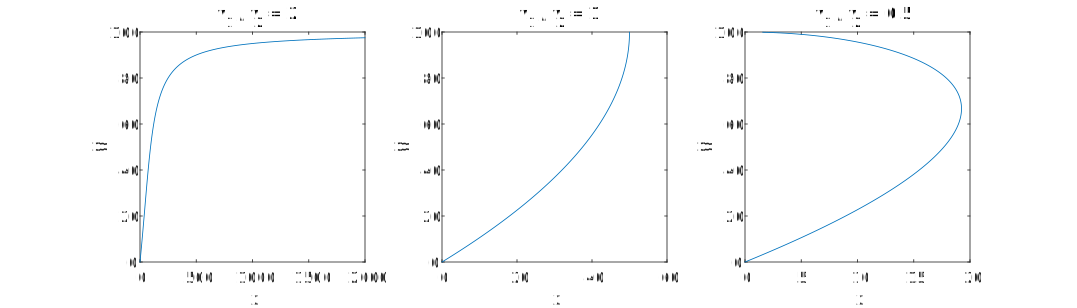
\includegraphics[width=\textwidth]{fig/ex6_analytical.pdf}
    \caption{当$k=v_1/v_2$取不同值时,小船航线的解析解。}
    \label{fig:ex6_analytical}
\end{figure}

\paragraph{数值解法} 可将\Cref{eq:ex6_dxy_dt}视为刚性方程,利用Matlab内置的\texttt{ode23s}方法求解即可。

\subsubsection{Matlab程序}

请参见\Cref{sec:ex6_code}。

\subsubsection{计算结果}

\paragraph{流速$v_1=0\ \mathrm{m/s}$时} 计算结果如\Cref{fig:ex6_v1_0}所示,小船渡河时间为$50\ \mathrm{s}$。

\paragraph{流速$v_1=0.5\ \mathrm{m/s}$时} 计算结果如\Cref{fig:ex6_v1_05}所示,小船渡河时间约为$54\ \mathrm{s}$。

\paragraph{流速$v_1=1\ \mathrm{m/s}$时} 计算结果如\Cref{fig:ex6_v1_1}所示,小船渡河时间约为$67\ \mathrm{s}$。

\paragraph{流速$v_1=1.5\ \mathrm{m/s}$时} 计算结果如\Cref{fig:ex6_v1_15}所示,小船渡河时间约为$114\ \mathrm{s}$。

\paragraph{流速$v_1=2\ \mathrm{m/s}$时} 计算结果如\Cref{fig:ex6_v1_2}所示,小船无限逼近终点,但始终不能到达,渡河所需时间为无穷大。

\begin{figure}
    \centering
    \subfigure[$x(t)$和$y(t)$图像]{
        \includegraphics[width=0.47\textwidth]{fig/ex6_v1_0_xtyt.pdf}
    }
    \subfigure[$x(y)$图像]{
        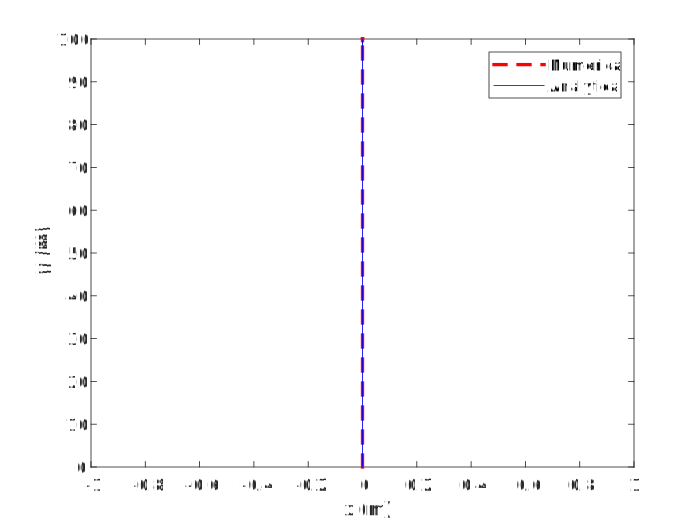
\includegraphics[width=0.47\textwidth]{fig/ex6_v1_0_xy.pdf}
    }
    \caption{流速$v_1=0\ \mathrm{m/s}$时,每一时刻的小船坐标$(x,y)$以及航线的数值结果。}
    \label{fig:ex6_v1_0}
\end{figure}

\begin{figure}
    \centering
    \subfigure[$x(t)$和$y(t)$图像]{
        \includegraphics[width=0.47\textwidth]{fig/ex6_v1_05_xtyt.pdf}
    }
    \subfigure[$x(y)$图像]{
        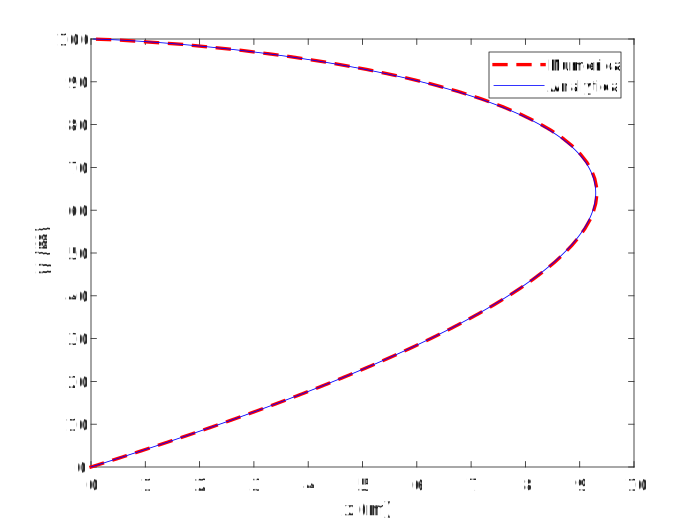
\includegraphics[width=0.47\textwidth]{fig/ex6_v1_05_xy.pdf}
    }
    \caption{流速$v_1=0.5\ \mathrm{m/s}$时,每一时刻的小船坐标$(x,y)$以及航线的数值结果。}
    \label{fig:ex6_v1_05}
\end{figure}

\begin{figure}
    \centering
    \subfigure[$x(t)$和$y(t)$图像]{
        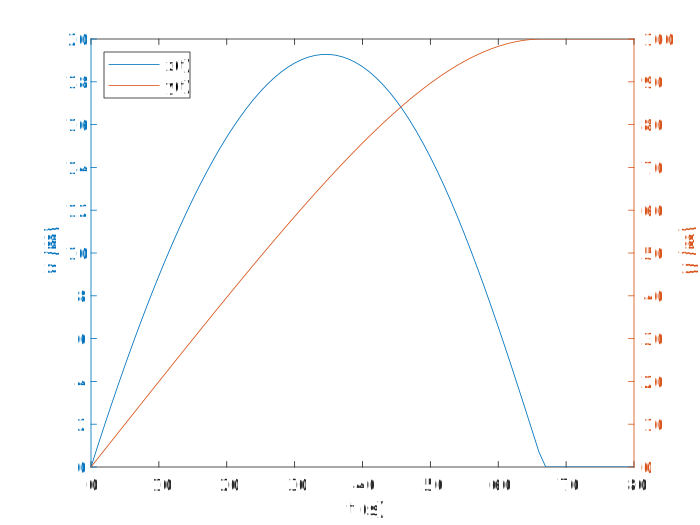
\includegraphics[width=0.47\textwidth]{fig/ex6_v1_1_xtyt.pdf}
    }
    \subfigure[$x(y)$图像]{
        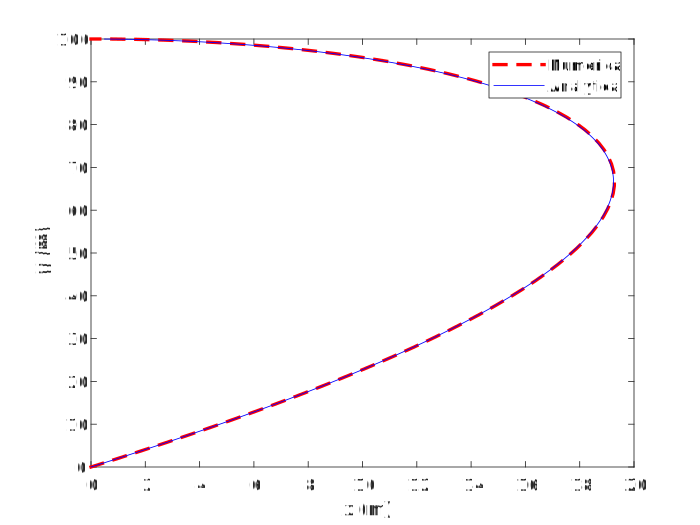
\includegraphics[width=0.47\textwidth]{fig/ex6_v1_1_xy.pdf}
    }
    \caption{流速$v_1=1\ \mathrm{m/s}$时,每一时刻的小船坐标$(x,y)$以及航线的数值结果。}
    \label{fig:ex6_v1_1}
\end{figure}

\begin{figure}
    \centering
    \subfigure[$x(t)$和$y(t)$图像]{
        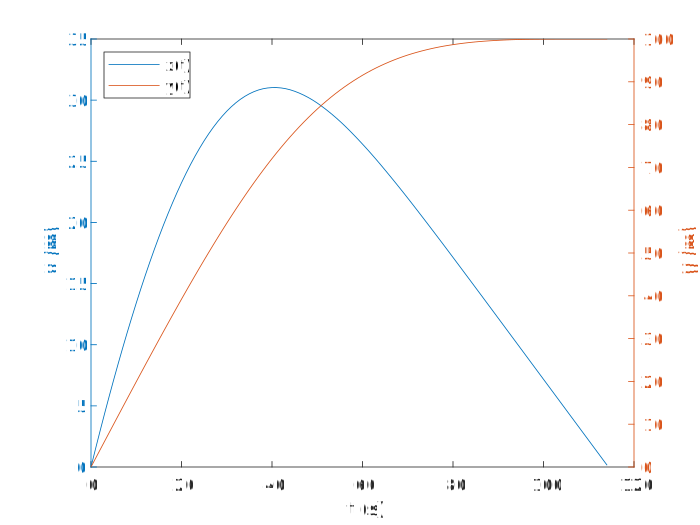
\includegraphics[width=0.47\textwidth]{fig/ex6_v1_15_xtyt.pdf}
    }
    \subfigure[$x(y)$图像]{
        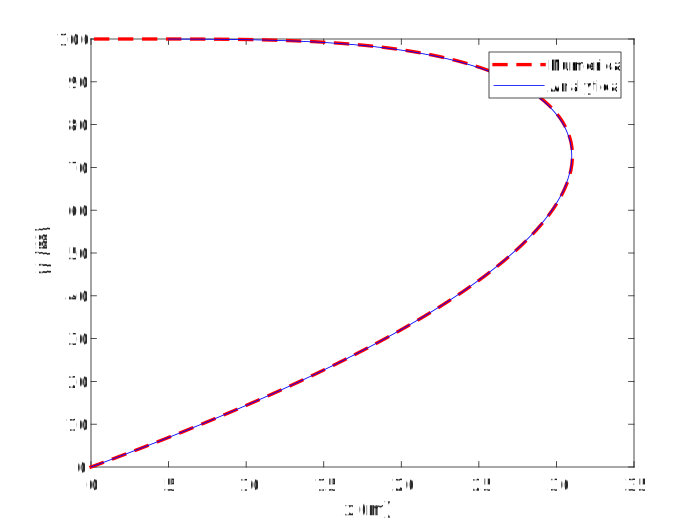
\includegraphics[width=0.47\textwidth]{fig/ex6_v1_15_xy.pdf}
    }
    \caption{流速$v_1=1.5\ \mathrm{m/s}$时,每一时刻的小船坐标$(x,y)$以及航线的数值结果。}
    \label{fig:ex6_v1_15}
\end{figure}

\begin{figure}
    \centering
    \subfigure[$x(t)$和$y(t)$图像]{
        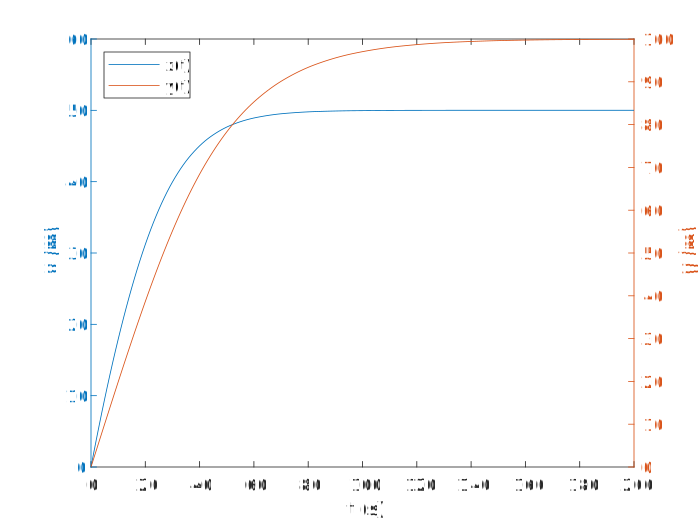
\includegraphics[width=0.47\textwidth]{fig/ex6_v1_2_xtyt.pdf}
    }
    \subfigure[$x(y)$图像]{
        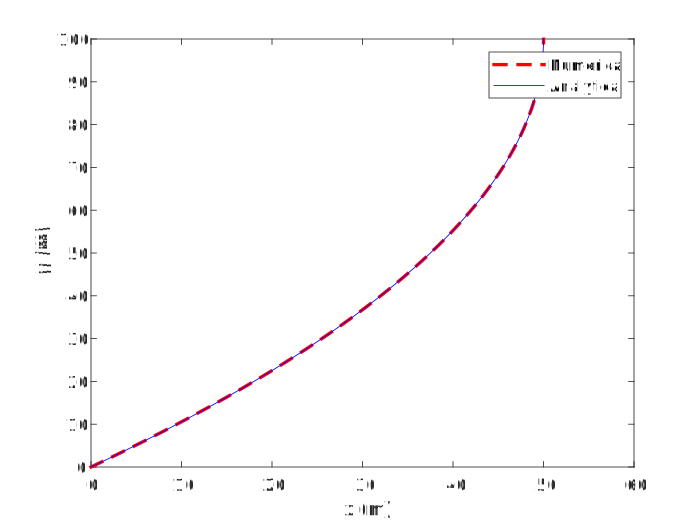
\includegraphics[width=0.47\textwidth]{fig/ex6_v1_2_xy.pdf}
    }
    \caption{流速$v_1=2\ \mathrm{m/s}$时,每一时刻的小船坐标$(x,y)$以及航线的数值结果。}
    \label{fig:ex6_v1_2}
\end{figure}

\subsubsection{结果分析}

数值结果的精度较高,与解析结果十分接近。从以上结果可以看出,当$v_1 < v_2$时,小船能够到达终点,且$v_1$越小,则渡河时间越短;当$v_1 = v_2$时,随着时间的流逝,小船无线逼近终点,但永远不能到达;当$v_1 > v_2$时,小船将随波逐流,离终点越来越远。

\subsubsection{结论}

当流速小于船速时,小船能够到达终点,且流速越小,小船渡河时间越短;当流速等于船速时,小船无线逼近终点,但永远不能到达;当流速大于船速时,小船将离终点越来越远。当流速分别为$0,0.5,1,1.5,2\ \mathrm{m/s}$时,小船渡河时间分别为$50,54,67,114,\infty\ \mathrm{s}$。

\subsection{Chap4-Ex9 种群竞争(计算题)}

\subsubsection{算法设计}

根据题目给出的种群竞争微分方程组模型,以及各小题给出的初值条件,利用Matlab内置的\texttt{ode45}求解即可。
\begin{equation}\label{eq:ex9_model}
    \frac{dx}{dt} = r_1x\left(1-\frac{x}{n_1}-s_1\frac{y}{n_2}\right), \quad
    \frac{dy}{dt} = r_2y\left(1-s_2\frac{x}{n_1}-\frac{y}{n_2}\right)
\end{equation}
其中$x(t),y(t)$分别为甲乙两个种群的数量,$r_1, r_2$为它们的固有增长率,$n_1, n_2$为它们的最大容量,$s_1$表示,对于供养甲的资源而言,单位数量乙的消耗是单位数量甲消耗的$s_1$倍,$s_2$同理。

\subsubsection{Matlab程序}

请参见\Cref{sec:ex9_code}。

\subsubsection{计算结果}

\paragraph{第1小题} 当$r_1=r_2=1,n_1=n_2=100,s_1=0.5,s_2=2,x_0=y_0=10$时,计算结果如\Cref{fig:ex9_sub1}所示,时间$t$充分大后,$x(t)$趋向于100,$y(t)$趋向于0。

\begin{figure}[t]
    \centering
    \subfigure[甲乙种群数量随时间变化的图像]{
        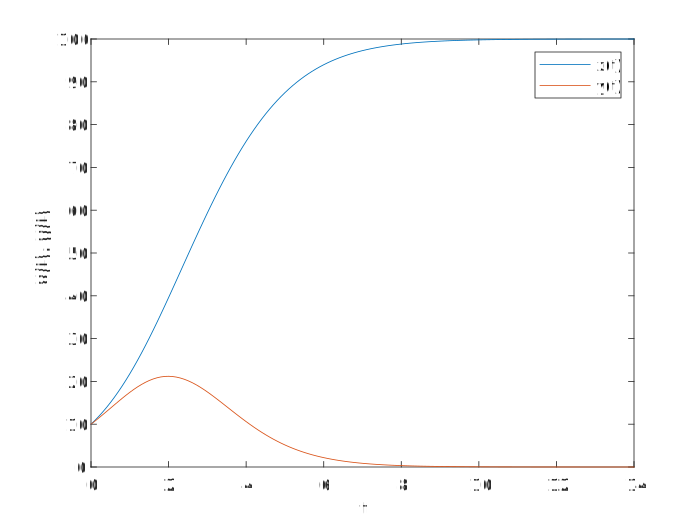
\includegraphics[width=0.47\textwidth]{fig/ex9_sub1.pdf}
    }
    \subfigure[甲乙种群数量的相图]{
        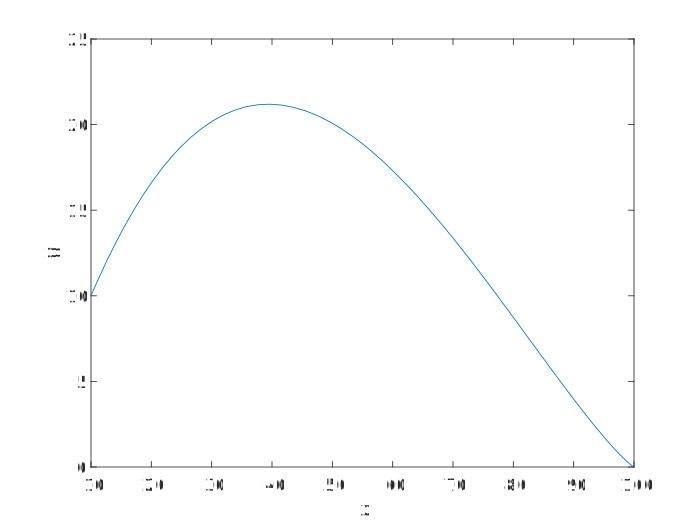
\includegraphics[width=0.47\textwidth]{fig/ex9_sub1_xy.pdf}
    }
    \caption{当$r_1=r_2=1,n_1=n_2=100,s_1=0.5,s_2=2,x_0=y_0=10$时,甲乙种群数量的图像和相图。}
    \label{fig:ex9_sub1}
\end{figure}

\paragraph{第2小题} 当$s_1 < 1$且$s_2 > 1$时,将参数重置为$r_1=1,r_2=2,n_1=200,n_2=300,s_1=0.5,s_2=2,x_0=20,y_0=100$,计算结果如\Cref{fig:ex9_sub2_bigx}所示。可以看出,当$s_1 < 1$且$s_2 > 1$时,时间充分大时,甲种群数量$x$趋向于$n_1$,乙种群数量$y$趋向于0,甲种群取代了乙种群。

\begin{figure}[t]
    \centering
    \subfigure[甲乙种群数量随时间变化的图像]{
        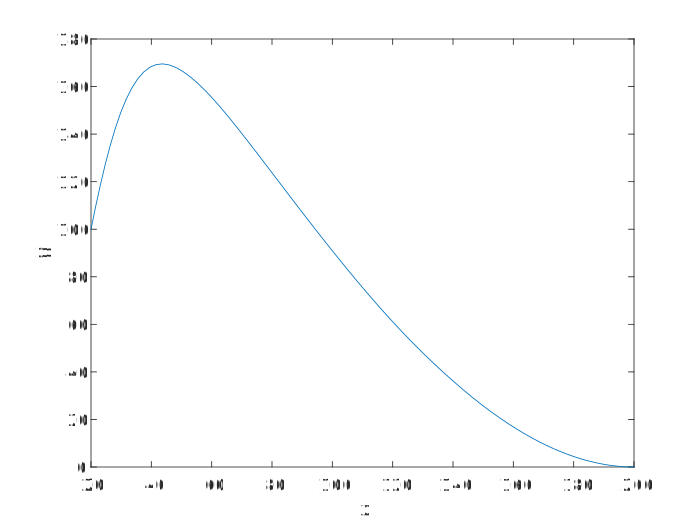
\includegraphics[width=0.47\textwidth]{fig/ex9_sub2_bigx_xtyt.pdf}
    }
    \subfigure[甲乙种群数量的相图]{
        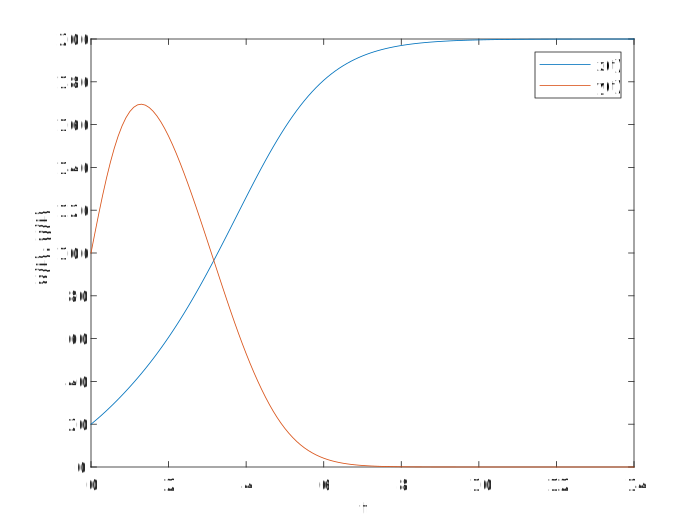
\includegraphics[width=0.47\textwidth]{fig/ex9_sub2_bigx_xy.pdf}
    }
    \caption{当$r_1=1,r_2=2,n_1=200,n_2=300,s_1=0.5,s_2=2,x_0=20,y_0=100$时,甲乙种群数量的图像和相图。}
    \label{fig:ex9_sub2_bigx}
\end{figure}

当$s_1 > 1$且$s_2 < 1$时,将参数重置为$r_1=1,r_2=2,n_1=400,n_2=300,s_1=1.5,s_2=0.7,x_0=200,y_0=100$,计算结果如\Cref{fig:ex9_sub2_bigy}所示。可以看出,当$s_1 > 1$且$s_2 < 1$时,时间充分大时,甲种群数量$x$趋向于0,乙种群数量$y$趋向于$n_2$,乙种群取代了甲种群。

\begin{figure}[t]
    \centering
    \subfigure[甲乙种群数量随时间变化的图像]{
        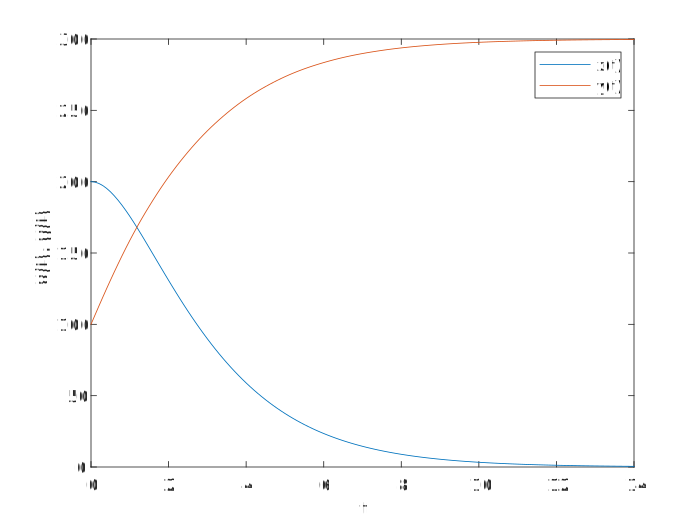
\includegraphics[width=0.47\textwidth]{fig/ex9_sub2_bigy_xtyt.pdf}
    }
    \subfigure[甲乙种群数量的相图]{
        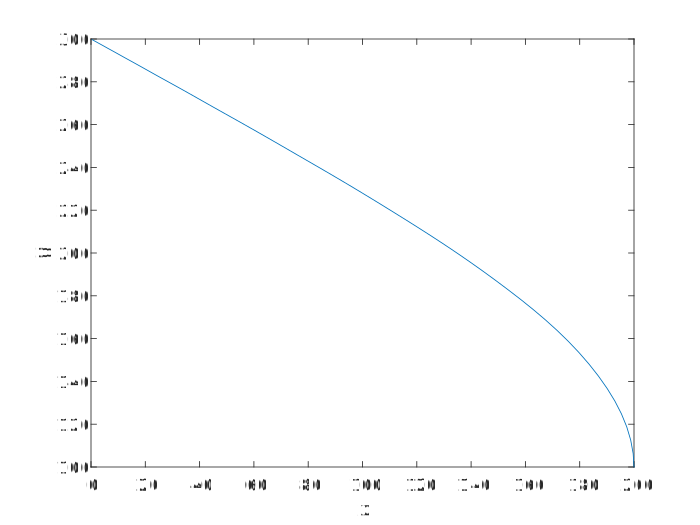
\includegraphics[width=0.47\textwidth]{fig/ex9_sub2_bigy_xy.pdf}
    }
    \caption{当$r_1=1,r_2=2,n_1=400,n_2=300,s_1=1.5,s_2=0.7,x_0=200,y_0=100$时,甲乙种群数量的图像和相图。}
    \label{fig:ex9_sub2_bigy}
\end{figure}

\paragraph{第3小题} 当$s_1<1,s_2<1$时,将参数重置为$r_1=1,r_2=2,n_1=400,n_2=300,s_1=0.8,s_2=0.7,x_0=200,y_0=100$,计算结果如\Cref{fig:ex9_sub3_bigy}所示。可以看出,当$s_1<1,s_2<1$时,时间充分大时,甲乙种群数量稳定在固定值,它们共同存在,不能完全取代对方。

\begin{figure}[t]
    \centering
    \subfigure[甲乙种群数量随时间变化的图像]{
        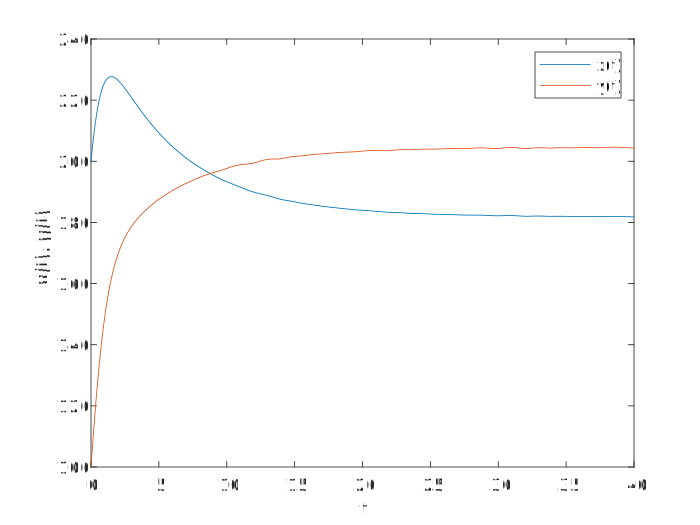
\includegraphics[width=0.47\textwidth]{fig/ex9_sub3_bigy_xtyt.pdf}
    }
    \subfigure[甲乙种群数量的相图]{
        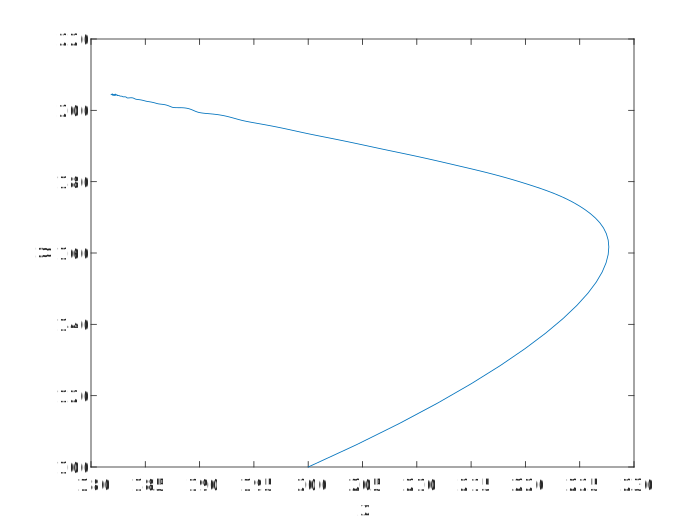
\includegraphics[width=0.47\textwidth]{fig/ex9_sub3_bigy_xy.pdf}
    }
    \caption{当$r_1=1,r_2=2,n_1=400,n_2=300,s_1=0.8,s_2=0.7,x_0=200,y_0=100$时,甲乙种群数量的图像和相图。}
    \label{fig:ex9_sub3_bigy}
\end{figure}

当$s_1>1,s_2>1$时,将参数重置为$r_1=1,r_2=2,n_1=400,n_2=300,s_1=1.5,s_2=1.7,x_0=200,y_0=100$,计算结果如\Cref{fig:ex9_sub3_bigx}所示。可以看出,时间充分大时,甲种群取代了乙种群;然而,当我将初值调整为$x_0=100,y_0=100$时,情况则完全相反,计算结果如\Cref{fig:ex9_sub3_unstable_bigy}所示。可以看出,时间充分大时,乙种群取代了甲种群。因此,当$s_1>1,s_2>1$时,模型是不稳定的,最终稳定状态的种群数量受初值条件的影响。

\begin{figure}[t]
    \centering
    \subfigure[甲乙种群数量随时间变化的图像]{
        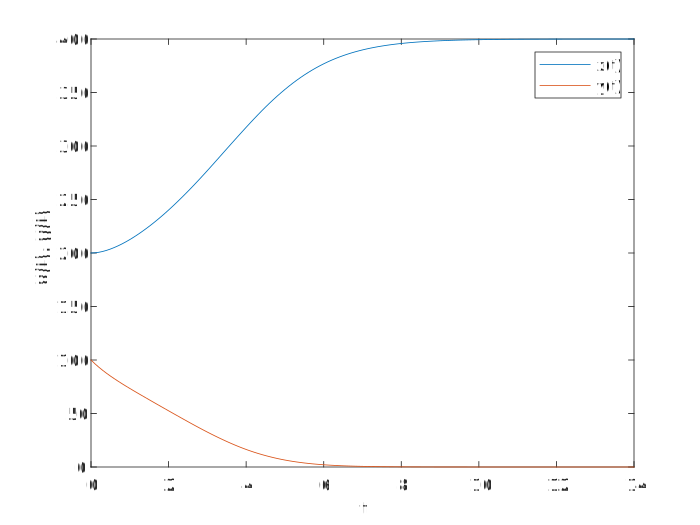
\includegraphics[width=0.47\textwidth]{fig/ex9_sub3_bigx_xtyt.pdf}
    }
    \subfigure[甲乙种群数量的相图]{
        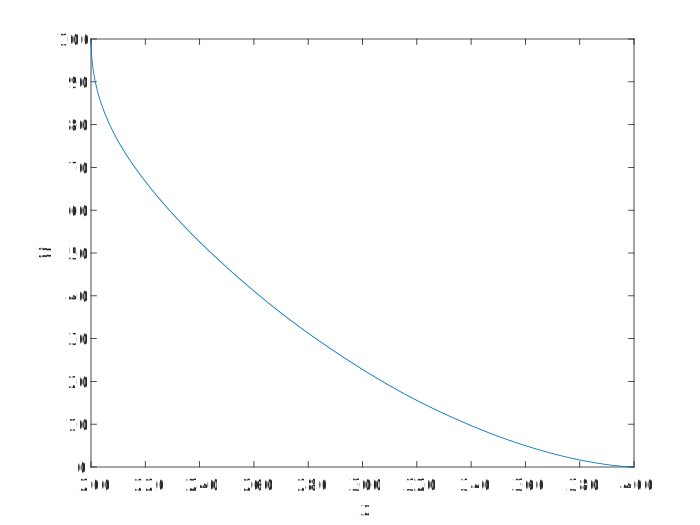
\includegraphics[width=0.47\textwidth]{fig/ex9_sub3_bigx_xy.pdf}
    }
    \caption{当$r_1=1,r_2=2,n_1=400,n_2=300,s_1=1.5,s_2=1.7,x_0=200,y_0=100$时,甲乙种群数量的图像和相图。}
    \label{fig:ex9_sub3_bigx}
\end{figure}

\begin{figure}[t]
    \centering
    \subfigure[甲乙种群数量随时间变化的图像]{
        \includegraphics[width=0.47\textwidth]{fig/ex9_sub3_unstable_bigy_xtyt.pdf}
    }
    \subfigure[甲乙种群数量的相图]{
        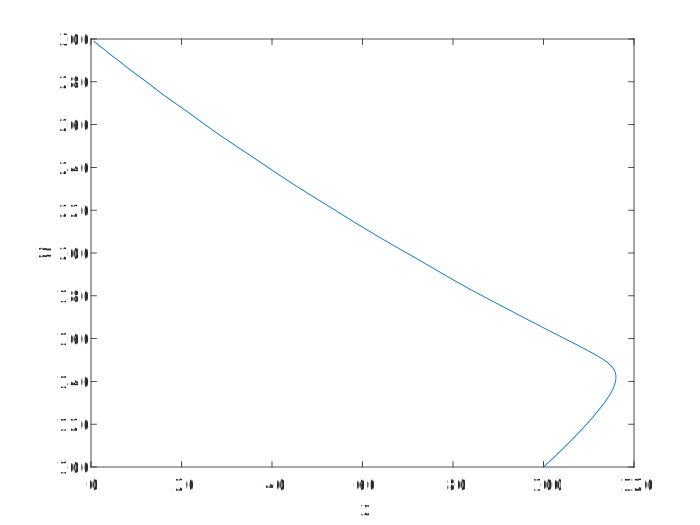
\includegraphics[width=0.47\textwidth]{fig/ex9_sub3_unstable_bigy_xy.pdf}
    }
    \caption{当$r_1=1,r_2=2,n_1=400,n_2=300,s_1=1.5,s_2=1.7,x_0=100,y_0=100$时,甲乙种群数量的图像和相图。}
    \label{fig:ex9_sub3_unstable_bigy}
\end{figure}

\subsubsection{结果分析}

由$x$和$y$的对称性,不妨假设$s_1 < s_2$,此时单位数量乙对供养甲的资源的消耗量比单位数量甲对供养乙的资源的消耗量更少,即甲的竞争能力相对更强。

当$s_1 < s_2 < 1$时,单位数量甲消耗供养乙的资源量为$s_2<1$,不及单位数量乙消耗供养乙的资源量,因此甲不能完全取代乙,随着时间的流逝,甲乙种群数量将趋于一个固定值,这个值可通过\Cref{eq:ex9_model}确定,令$dx/dt=0,dy/dt=0$,注意到此时$x\ne 0, y\ne 0$,可解得稳态时甲乙种群数量如下式,与数值计算结果相符。
\begin{equation}
    \lim_{t\rightarrow +\infty}x(t)=n_1\frac{1-s_1}{1-s_1s_2},\quad
    \lim_{t\rightarrow +\infty}y(t)=n_2\frac{1-s_2}{1-s_1s_2}
\end{equation}

当$s_1 < 1 < s_2$时,在时间足够长时,由于甲的竞争力太强,而乙的竞争力太弱,因此甲最终会取代乙。

当$1 < s_1 < s_2$时,模型不稳定,最终稳定状态的种群数量受初值条件的影响。

\subsubsection{结论}

当$s_1 < s_2 < 1$时,最终甲乙种群共存;当$s_1 < 1 < s_2$时,最终甲会取代乙;当$1 < s_1 < s_2$时,模型不稳定,最终状态受初值条件的影响。

\section{收获与建议}

在本次实验中,我通过使用Matlab,掌握了求微分方程初值问题数值解的方法,用微分方程模型解决了简化的实际问题,了解了欧拉方法和龙格-库塔方法的基本思想和计算公式,在解决实际问题的过程中,我对数学方法的原理和应用有了更深刻的理解。

希望助教能对每次的实验进行详细的解答,希望老师在未来的课堂上介绍更多数学应用的前沿知识。

\section{附录:Matlab程序代码}

\subsection{Chap4-Ex5}\label{sec:ex5_code}

\lstinputlisting[language=Matlab]{../src/ex5.m}

\subsection{Chap4-Ex6}\label{sec:ex6_code}

\lstinputlisting[language=Matlab]{../src/ex6.m}

\subsection{Chap4-Ex9}\label{sec:ex9_code}

\lstinputlisting[language=Matlab]{../src/ex9.m}

\end{document}
